% !TeX spellcheck = es_ES 
\documentclass{article}

\usepackage[section]{placeins}
\usepackage{enumerate}
\usepackage{makecell} 
\usepackage{graphicx}
\usepackage{url}
\usepackage[spanish]{babel}
\usepackage[utf8]{inputenc}
\usepackage[backend=biber, style=numeric]{biblatex}
\addbibresource{ProtocoloRSL.bib}

\begin{document}

  \title{%
  Protocolo de trabajo\\
  \large Revisión de la literatura sobre las actividades de requisitos para Software como Servicio\\}
  \author{Alberto de Jesús Sánchez López \\ 
  \small Proyecto Guiado}
  \author{\makebox[.9\textwidth]{Alberto de Jesús Sánchez López }\\Universidad Veracruzana \and M.C.C.María Angélica Cerdán \and Dr.Jorge Octavio Ocharán Hernández}
  \author{\makebox[.6\textwidth]{Alberto de Jesús Sánchez López}\\Universidad Veracruzana\\ \and M.C.C. María Angélica Cerdán \and Dr. Jorge Octavio Ocharán Hernández}
  \date{Fecha}
  \maketitle
  \thispagestyle{empty}
  \newpage

  \tableofcontents
  \thispagestyle{empty}
  \newpage

\setcounter{page}{1}
\section{Antecedentes}

El concepto de rentar recursos computacionales como servicio, fue introducido en 1971 a la industria por IBM (de sus siglas en inglés International Business Machine) y RJE, empresa de manufactura de microprocesadores que 
trabajaba para IBM. En aquel momento, el término se denominó “time-sharing” (White 1971). Con el transcurrir del tiempo, la adopción de esta modalidad de distribución ha provocado un cambio importante en la forma 
de adquisición de bienes en Internet, motivando el surgimiento de proveedores en servicios digitales dinámicos, que proveen funcionalidades y modelos de pago flexibles, así como un proceso de adquisición totalmente 
automático (autoservicio), donde la disposición del recurso debe ser ejecutada, otorgada y administrada en su totalidad en línea.

A este modelo aplicado al software, se le llama SaaS (por sus siglas en inglés Software as a Service), que ha sido ampliamente adoptado debido a que permite una economía de escala en el desarrollo de software y al nivel 
de acceso que permite un modelo que se ejecuta en la nube, lo que hace conveniente la adquisición bajo este formato. Dentro del primer trimestre del año en curso, se observó un crecimiento del 30%
en el porcentaje promedio de ventas anuales, producido por aplicaciones SaaS de tipo empresarial en el mercado global, según Microsoft (Spencer 2020). Otro estudio revela que algunos de los factores más influyentes en el 
proceso de adopción de software como servicio, es el manejo de seguridad y privacidad de los datos, la ventaja competitiva de adquirir software que ha pasado bajo un proceso de validación, así como una adopción de cultura orientada a la comunicación.

La tendencia a adoptar trabajo en casa y educación línea, causado por la pandemia, ocasionada por el virus Sars-COV2, motivará un crecimiento en el desarrollo de aplicaciones orientadas al SaaS (Smith 2020). Esto hace 
surgir una necesidad a aquellos interesados sobre la información relacionada al desarrollo de un Software como Servicio.
Como todo proceso de desarrollo de un sistema de software, no es una actividad sencilla, sigue las fases convencionales reconocidas en el campo de la Ingeniería de Software y puede aplicar estándares internacionales 
que definen el ciclo de vida del software, sin embargo, este tipo de aplicaciones enfrentan condiciones relativas a su propia naturaleza, que motivan la adaptación de los procesos básicos pertenecientes al desarrollo de software 
tradicional, así como el estudio de los métodos que se utilizan dentro del mismo.


Un área de especial interés, es la definición y administración de requisitos, un requisito es determinado como “Descripciones de los servicios que un sistema debería proveer y las restricciones en su operación… El proceso de encontrar, analizar, 
documentar y verificar los servicios y restricciones de un sistema es llamado Ingeniería de requisitos” (Sommerville, 2016, 102). Es decir, la fase de definición de requisitos es un proceso complejo y con gran importancia en el ciclo 
de vida de un producto de software, puesto que una definición detallada de los requisitos influye en la calidad del producto final, por ende, la especificación de los requisitos, debe ser un artefacto producido mediante un 
proceso bien delimitado, planeado, probado y medido. Si la especificación de requisitos ha sido resultado de un proceso formal, la probabilidad de que el proyecto sea un éxito, aumenta (Anton 2003).

Para llevar a cabo un proceso de desarrollo de software que asegure calidad en el producto final, es importante una fase de definición de requisitos de software sólida (Hussain and Mkpojiogu 2016), años de investigación y 
experiencia recabada por la comunidad, ha hecho que el desarrollo de requisitos para sistemas tradicionales sea un tema basto en información, lo que facilita el proceso de planeación de una elicitación.

Pero la definición de requisitos para un Software como Servicio, está muy lejos de ser tradicional (Anum Tariq, Dr. Shoab Ahmed Khan Sundas Iftikhar, n.d.), en esta área relativamente nueva, es fundamental analizar la 
información disponible relacionada al tema y plantear una propuesta que se apegue a las necesidades especiales del desarrollo de un SaaS. 

Definir un proceso para recolectar información sobre las metodologías, estrategias y herramientas utilizadas en el proceso de requisitos en un SaaS, no es una tarea sencilla, debido a que la información existe, 
pero está dispersa, no hay una clasificación formal sobre la misma y no existe una compilación sobre la información actual el tema. Esto es de gran interés para aquellos desarrolladores e investigadores interesados 
en el área, ya que existen múltiples estrategias utilizadas para el desarrollo de requisitos en sistemas tradicionales, no obstante, en sistemas en los que existe una necesidad general a cubrir o un conjunto de 
clientes con una necesidad en común, pero con detalles específicos, se presentan complejidades que necesitan atención especial. 
 
Esto genera una necesidad para cerrar la brecha de conocimiento dentro del área, por medio de una Revisión Sistemática de la Literatura sobre el estado del arte de la fase de requisitos para el Software como Servicio, la 
cual proveerá punto de inicio para aquellos interesados en la información y una clasificación sobre la misma.
\newpage

\section{Planteamiento del Problema}
Con la adopción del Saas en la industria, ha surgido la necesidad de investigar y analizar su elaboración, en este caso, en la definición de requisitos, una fase crítica para el aseguramiento de calidad de cualquier 
producto de software. Actualmente existen propuestas documentadas relacionadas al desarrollo de Software como Servicio, pero la información disponible está dispersa, no está centrada sobre el proceso de 
definición de requisitos y no existe una compilación sobre el estado del arte en métodos existentes, esto provoca la falta de dirección clara para investigaciones en el área. Por lo que, el problema que 
motiva el presente trabajo se puede enunciar de la siguiente forma:\\

\textbf{No existe un análisis sobre el estado del arte del proceso de definición de requisitos en un Software como Servicio.}\\

Lo anterior es un obstáculo para aquellos investigadores interesados en el área, o para equipos de desarrollo que busquen iniciar la definición de necesidades del cliente, con información recopilada siguiendo un proceso formal. 
Esto causa cierta urgencia en la investigación dentro del tema, ya que, una definición de requisitos sólida es fundamento vital para la toma de decisiones dentro de cualquier proyecto de desarrollo de software, 
en especial cuando no existe un cliente en particular o se tiene que llenar una necesidad dentro de un mercado, siendo el riesgo más alto, si la inversión no ofrece rentabilidad y cobertura sobre la tasa de retorno. 

Para realizar un análisis del estado del arte sobre la fase de requisitos de un Software como Servicio, es necesario realizar las siguientes tareas:

Definir una metodología para recopilar y analizar la información del estado del arte de la fase de los requisitos de un software como servicio, siguiendo un proceso científico.
Compilar la información sobre los métodos, técnicas y herramientas aplicados en la fase de requisitos de un software como servicio.
Identificar las tendencias y temas abiertos en cuanto a métodos, técnicas y herramientas para la fase de requisitos de la ingeniería de software como servicio.

Con esto, se pretende abordar la falta de una compilación de métodos existentes que dificulta la proyección de tendencias para las siguientes investigaciones. 

\newpage

\section{Objetivos}
\textbf{Objetivo general} \\

Analizar el estado del arte sobre el proceso de requisitos en el desarrollo de Software como servicio a través de una revisión sistemática de literatura, para identificar temas abiertos en el área disciplinar. \\

\textbf{Objetivos específicos} \\

\begin{itemize}
    \item Establecer las preguntas de investigación que permitan analizar el estado del arte sobre el proceso de requisitos en el desarrollo de software como servicio, que deberán ser respondidas por la revisión sistemática de literatura.
    \item Realizar una búsqueda de literatura especializada en bases de datos confiables, aplicando criterios de inclusión de exclusión para determinar los documentos a analizar.
    \item Extraer información relevante de los documentos seleccionados de la literatura especializada, a través de una matriz de extracción que permita el análisis de métodos, técnicas y herramientas aplicadas en el proceso de requisitos en el desarrollo de software como servicio.
    \item Aplicar una técnica de metaanálisis para contrastar y combinar las propuestas de los diferentes estudios contenidos en la literatura especializada para el proceso de requisitos en el desarrollo de software como servicio.
    \item Identificar las tendencias en las propuestas analizadas de la literatura especializada para determinar los temas abiertos en el área disciplinar de los procesos de requisitos en el desarrollo de software como servicio.
\end{itemize}

\newpage

\section{Justificación}

Actualmente, no existe una Revisión Sistemática de la Literatura orientada hacia conocer el estado estado del arte sobre las actividades de requisitos realizadas para un Software como Servicio, 
realizar un análisis sobre las actividades y metodologías, sería de gran ayuda para investigadores interesados en el área, ofrecer un conjunto de propuestas de investigación para investigaciones futuras. 
Todo lo anterior es vital para avanzar el conocimiento actual dentro del área, ya que la información compilada habría pasado por un filtro de calidad, habría sido previamente organizada y clasificada 
según el método, lo cual facilita el proceso para investigación sobre el tema. 

Realizar la Revisión Sistemática de Literatura permitiría lo siguiente: 

\begin{itemize}
    \item Desarrollar una compilación sobre los métodos para identificar el estado de arte actual en definición de requisitos para Software como Servicio.
    \item Definir una clasificación estructurada con el fin conocer las áreas de mejor desempeño para los métodos, herramientas y estrategias encontrados.
    \item Brindar una compilación actual, creada siguiendo una metodología científica, sobre el estado del arte sobre la fase de requisitos en el Software como Servicio.
    \item Proponer áreas de investigación potenciales en la fase de requisitos en el Software como Servicio.
\end{itemize}
\newpage

\section{Alcances y Limitaciones}
\textbf{Alcances} \\
Se realizará una revisión sistemática de la literatura para documentar el estado actual de las actividades 
empleadas en el proceso de requisitos para un software como servicio, 

\textbf{Limitaciones} \\

\newpage

\section{Marco Teórico}
\newpage

\section{Método}
Se utilizará una revisión sistemática de la literatura como método para llevar a cabo esta investigación, 
empleando la guía de Kitchenham y Charters. Donde se especifican preguntas de investigación que tienen 
como objetivo dirigir la investigación, después se determina una estrategia para la selección y búsqueda de estudios para 
terminar el proceso con una síntesis de la información encontrada, para ello se seleccionó la síntesis narrativa, utilizando como 
modelo la guía por \cite{sintesisnarrativa} 

\begin{figure}[!htb]
   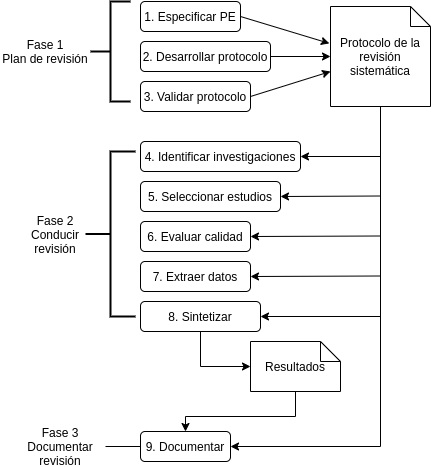
\includegraphics[width=\linewidth]{metodo.png}
   \caption{Visión general del método para la revisión sistemática de la literatura.}
   \label{fig:etapasconducción}
\end{figure}

\newpage

\section{Cronograma}
Se diseñó un cronograma, que contiene el conjunto de actividades clave para completar la revisión sistemática de la literatura, 
con el propósito de determinar tiempos de ejecución, documentar las tareas a llevar a cabo y asignar espacios de tiempo apropiados 
para completar la revisión en el periodo designado. Para realizar lo anterior es necesario calcular las horas totales necesarias para completar el proyecto. 
La formula utilizada para calcular el total de trabajo, fué extraído de REFERENCIA,

\newpage

\section{Referencias}
\printbibliography

\end{document}
